% !TEX root = ../phd-thesis.tex

\chapter{Local Completeness Logic}\label{ch:lcla}
In this chapter, we extend $\LCLA$ (see Section~\ref{sec:sota:lcl}) with new capabilities. First, we investigate the possibility of relaxing point (3) of Theorem~\ref{th:sota:lcl-soundness} to $\denot{\regr}^{A} \alpha(P) = \alpha(Q)$ to achieve extensional soundness, i.e., to untie the set of properties that can be proved about the function computed by the program from the way the program is written. To do so, we follow the idea introduced in~\cite[§8]{BGGR23} of \emph{changing the abstract domain} during the analysis, possibly in different ways for different portions of the code.
While~\cite{BGGR23} proposes a single rule for domain refinement, we study here both \emph{refinement} and \emph{simplification} rules for $\LCLA$.
Moreover, we study here how to weaken the hypothesis of Galois connection: the whole theory of completeness is based on the existence of a best approximation for concrete points, but this is not always available in practical instances~\cite{CC92}.
Lastly, we study further the possibility of using $\LCLA$ for backward analysis, as briefly outlined in~\cite[\S 5.3]{BGGR23}.

The content of this chapter is based on~\cite{ABG23} and~\cite[\S 6]{ABGL24}.

\section{Motivation}
While any $\LCLA$ valid triple allows to prove both correctness and incorrectness, a very powerful ability, proving an $\LCLA$ triple can be challenging. Therefore, it is important to study how to simplify this task.

The strongest of the three properties required by $\LCLA$ is point~(3) in Theorem~\ref{th:sota:lcl-soundness}, which in turn is key to guarantee that point~(2) holds.
However, requiring the abstract interpreter $\denot{\regc}^{\sharp}_{A}$ to be locally complete is an \emph{intensional} property, because the function $\denot{\regc}^{\sharp}_{A}$ depends on how $\regc$ is written.
In fact, it is well known that the abstract analyses $\denot{\regc_1}^{\sharp}_{A}$ and $\denot{\regc_2}^{\sharp}_{A}$ of two programs $\regc_1$ and $\regc_2$ computing the same function (i.e., $\denot{\regc_1}=\denot{\regc_2}$) can yield different results.

A weaker requirement that suffices to guarantee the validity of point~(2) is the local completeness of the bca $\denot{\regc}^{A}$ of the function $\denot{\regc}$, which is an \emph{extensional} property: it only depends on the abstract domain $A$ and on the computed function $\denot{\regc}$ associated with $\regc$, not on the way $\regc$ is composed. In its original formulation, $\LCLA$ exploits $\denot{\regc}^{\sharp}_{A}$ instead of $\denot{\regc}^{A}$ because the second can be as hard to compute as the concrete semantics $\denot{\regc}$ and because the sequential composition of bcas is not necessarily a bca itself.
The difference between $\denot{\regc}^{A}$ and $\denot{\regc}^{\sharp}_{A}$ is exemplified below (see also, e.g.,~\cite[Example~1]{LL09}):

\begin{example}[Extensional and intensional properties]\label{ex:lcla:ext-vs-int}
	Consider the concrete domain $\pow(\setZ)$ of sets of integers and the abstract domain of signs given below:
	\begin{center}
		% \begin{tikzpicture}
		% 	\draw (-1,0) node[name=1] {\footnotesize$\varnothing$};
		% 	\draw (-2,1) node[name=2] {\footnotesize$\setZ_{<0}$};
		% 	\draw (-1,1) node[name=3] {\footnotesize$\setZ_{=0}$};
		% 	\draw (0,1) node[name=4] {\footnotesize$\setZ_{>0}$};
		% 	\draw (-2,2) node[name=5] {\footnotesize$\setZ_{\leq 0}$};
		% 	\draw (-1,2) node[name=8] {\footnotesize$\setZ_{\neq 0}$};
		% 	\draw (-0,2) node[name=6] {\footnotesize$\setZ_{\geq 0}$};
		% 	\draw (-1,3) node[name=7] {\footnotesize$\setZ$};
		% 	\draw (-3.5,2.9) node[name=n] {{\normalsize $\Sign$}};
		%
		%
		% 	\draw[semithick] (1) -- (2);
		% 	\draw[semithick] (1) -- (3);
		% 	\draw[semithick] (1) -- (4);
		% 	\draw[semithick] (2) -- (5);
		% 	\draw[semithick] (2) -- (8);
		% 	\draw[semithick] (3) -- (5);
		% 	\draw[semithick] (3) -- (6);
		% 	\draw[semithick] (4) -- (6);
		% 	\draw[semithick] (4) -- (8);
		% 	\draw[semithick] (5) -- (7);
		% 	\draw[semithick] (6) -- (7);
		% 	\draw[semithick] (8) -- (7);
		% \end{tikzpicture}
		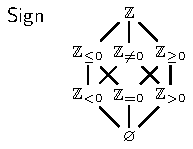
\includegraphics{sign-domain.pdf}
	\end{center}
	The meaning of each abstract elements of $\Sign$ is to represent concrete values that satisfy the respective property: for instance, $\gamma(\setZ_{< 0}) = \{ n \in \setZ \svert n < 0 \}$ and $\alpha( \{ 0; 1; 100 \}) = \setZ_{\ge 0}$.
	The bca of a concrete function $f: \pow(\setZ) \to \pow(\setZ)$ is defined as $f^{\Sign}\eqdef \alpha~f~\gamma: \Sign \to \Sign$.

	Consider the simple program fragment
	$$\regc \eqdef \code{x := x + 1; x := x - 1}\ .$$

	It's denotational semantics $\denot{\regc}$ is the identity $\id_{\setZ}$, so its bca (see Definition~\ref{def:bg:sound-abstraction})
	\[
	\denot{\regc}^{\Sign} \eqdef \alpha~\id_{\setZ}~\gamma = \id_{\Sign}
	\]
	is just the abstract identity. We say that $\denot{\regc}^{\Sign}$ is \emph{extensional} because it only depends on the function computed by $\regc$, i.e., its denotational semantics. However, an analyser does not know the semantics of $\regc$, so it has to analyse the program syntactically, breaking it down into elementary pieces and gluing the results together. For instance, starting from the concrete point $P = \{ 1 \}$, the analysis first abstracts it to the property $\alpha(P) = \setZ_{> 0}$, then it computes
	\begin{align*}
		\denot{\regc}^{\sharp}_{\Sign} (\setZ_{> 0}) & = \denot{\code{x := x - 1}}^{\sharp}_{\Sign} \denot{\code{x := x + 1}}^{\sharp}_{\Sign} (\setZ_{> 0}) \\
		                                             & = \denot{\code{x := x - 1}}^{\sharp}_{\Sign} (\setZ_{> 0}) = \setZ_{\ge 0} .
	\end{align*}
	Analogous calculations for all properties in $\Sign$ yields the abstraction
	\[
	\denot{\regc}^{\sharp}_{\Sign}(a) = \begin{cases*}
		\varnothing   & if $a = \varnothing$                                                                                     \\
		\setZ_{\ge 0} & if $a \in \{ \colorbox{lightgray}{$\setZ_{= 0}$}, \colorbox{lightgray}{$\setZ_{> 0}$}, \setZ_{\ge 0} \}$ \\
		\setZ_{< 0}   & if $a = \setZ_{< 0}$                                                                                     \\
		\setZ         & if $a \in \{ \colorbox{lightgray}{$\setZ_{\le 0}$}, \colorbox{lightgray}{$\setZ_{\neq 0}$}, \setZ \}$
	\end{cases*}
	\]
	that, albeit sound, is less precise than $\id_{\Sign}$ (we highlight with a gray background all inputs on which $\denot{\regc}^{\sharp}_{\Sign}$ loses accuracy).

	The program $\regc$ is equivalent to the command $\code{skip}$, because $\denot{\code{skip}}=\id_{\setZ}$, and thus $\regc$ and $\code{skip}$ are assigned the same bca $\denot{\code{skip}}^{\Sign} = \denot{\regc}^{\Sign} = \id_{\Sign}$.
	However, $\denot{\code{skip}}^{\sharp}_{\Sign} = \id_{\Sign} \neq \denot{\regc}^{\sharp}_{\Sign}$, exposing the \emph{intensional} essence of the abstract interpreter: the abstraction depends on how the program is written and not only on its semantics.\footnote{While it falls outside the scope of this thesis, we refer the interested reader to, e.g.,~\cite{BGGGP19,BRZ22} for more about intensional and extensional abstract properties.}
\end{example}

The possibility of weakening point~(3) from being an intensional requirement based on $\denot{\regc}^{\sharp}_A$ to an extensional one based on bcas $\denot{\regc}^A$ has several nice consequences.
First, the local completeness of $\denot{\regc}^A$ is enough to guarantee that points~(1-2) hold.
Second, while the proof system itself provides an intensional analysis, because its rules are defined inductively on the program syntax, the information it produces is more precise, in the sense that the property associated with triples is extensional: no precision is lost because of the approximation introduced by the intensional abstract interpreter.
Third, it allows the proof system to derive more triples than the original one because a bca can be locally complete even when the abstract interpreter is not (but not vice versa).
Finally, since extensional properties are independent of how the program is written, this possibility provides the potential for deriving exactly the same triples for equivalent programs.

Another constraint imposed by $\LCLA$ is the need for a Galois connection: the whole theory of completeness in abstract interpretation is based on it. Therefore, $\LCLA$ cannot be applied to known instances of abstract domains lacking an abstraction function $\alpha$, such as convex polyhedra~\cite{CH78} that are widely used in static analysis. However, abstract convexity of local completeness can help mitigate this limitation: even if a point doesn't have a best abstraction, if it can be bound between another point and its abstraction, we can in a sense ``prove'' local completeness on it thanks to abstract convexity.

Lastly, $\LCLA$ was proposed for forward analysis. In theory, nothing prevents it to be used in a backward fashion, but the classical forward/backward duality requires the use of under-approximation abstract domains, making it impractical (see Chapter~\ref{ch:uai}). However, if we consider the backward semantics $\bwsem{\cdot}$ defined in the previous chapter, it turns out that it is possible to combine SIL (Section~\ref{sec:sil:sil}) with over-approximation abstract domain in a $\LCLA$-style.

\section{Extensional soundness}
As anticipated at the beginning of the chapter, one of our goals is to weaken point (3) of the soundness Theorem~\ref{th:sota:lcl-soundness} from local completeness of the abstract interpreter $\denot{\regr}^{\sharp}_A$ to that of the bca $\denot{\regr}^A$. The key observation is that the proof of Corollary~\ref{th:sota:corollary-verification} only relies on points (1-2) of Theorem~\ref{th:sota:lcl-soundness}, so from a program analysis perspective point (3) can be seen as a technical requirement to prove the other two. However, we observe that local completeness of the bca is enough to this aim: we therefore present a slightly weaker\footnote{Logically speaking, we prove a stronger conclusion, so the theorem as an implication is weaker.} soundness result for $\LCLA$, with the bca $\denot{\regr}^A$ in place of the inductively defined abstract interpreter $\denot{\regr}^{\sharp}_A$.

\begin{theorem}[Extensional soundness]\label{th:lcla:soundness-ext}
	Let $A_{\alpha, \gamma} \in \Abs(C)$.
	If $\lcl{A}{P}{\regr}{Q}$ then:
	\begin{enumerate}
		\item $Q \le \denot{\regr} P$,
		\item $\alpha(\denot{\regr} P) = \alpha(Q)$,
		\item $\denot{r}^A \alpha(P) = \alpha(Q)$.
	\end{enumerate}
\end{theorem}
\begin{proof}
	First we remark that points (1) and (3) implies point (2):
	\begin{align*}
		\alpha(Q) & \le \alpha(\denot{\regr} P)     & [\text{(1) and monotonocity of }\alpha] \\
		          & \le \denot{\regr}^{A} \alpha(P) & [\text{soundness of }\denot{\regr}^{A}] \\
		          & = \alpha(Q)                     & [\text{(3)}]
	\end{align*}
	So all the lines are equal, in particular $\alpha(Q) = \alpha(\denot{\regr} P)$.
	The proof is then by induction on the derivation tree of $\lcl{A}{P}{\regr}{Q}$, but we only have to prove (1) and (3) because of the observation above.
	We only include one inductive case as an example; the full proof is in Appendix~\ref{ch:app:lcla}.

	\proofcase{\lclrule{seq}}
	\noindent (1) $Q \le \denot{\regr_2} R \le \denot{\regr_2} (\denot{\regr_1} P) = \denot{\regr1; \regr_2} P$, where the inequalities follow from inductive hypotheses and monotonicity of $\denot{\regr_2}$.

	\noindent (3) We recall that $\denot{\regr_1; \regr_2}^{A} \le \denot{\regr_2}^{A} \denot{\regr_1}^{A}$.
	\begin{align*}
		\alpha(Q) & \le \alpha(\denot{\regr_1; \regr_2} P)                & [\text{(1) and monotonicity of }\alpha] \\
		          & \le \denot{\regr_1; \regr_2}^{A} \alpha(P)            & [\text{soundness of }\denot{\regr}^{A}] \\
		          & \le \denot{\regr_2}^{A} \denot{\regr_1}^{A} \alpha(P) & [\text{recalled above}]                 \\
		          & = \denot{\regr_2}^{A} \alpha(R)                       & [\text{inductive hp}]                   \\
		          & = \alpha(Q)                                           & [\text{inductive hp}]
	\end{align*}
	So all the lines are equal, in particular $\denot{\regr_1; \regr_2}^{A} \alpha(P) = \alpha(Q)$.
\end{proof}

Theorem~\ref{th:sota:lcl-soundness} involves $\denot{\regr}^{\sharp}_A$, an \emph{intensional} property of the program $\regr$ that depends on how the program is written, while the new statement we propose here relies only on $\denot{\regr}^A$, an \emph{extensional} property of the computed function $\denot{\regr}$ and not of $\regr$ itself.
Accordingly, for the rest of this chapter we use the name \emph{intensional soundness} for the former and \emph{extensional soundness} for the latter.
Again, we say a triple is \emph{extensionally valid} if it satisfies point (1--3) of Theorem~\ref{th:lcla:soundness-ext} above, and intensionally valid for the former notion introduced in Section~\ref{sec:sota:lcl}. We shall write $\lclvalid{A}{P}{\regr}{Q}$ for both, but we will make sure to disambiguate the notation when not clear from the context.

\section{Locally complete refinement}
\begin{figure*}[t]
	\begin{framed}
		\[
		\infer[\lclrule{refine\mbox{-}ext}]
		{\lcl{A}{P}{\regr}{Q}}
		{\lcl{A'}{P}{\regr}{Q} & A' \preceq A & A \denot{\regr}^{A'} A(P) = A(Q)}
		\]
	\end{framed}
	\vspace{-1ex}
	\caption{Rule \lclrule{refine\mbox{-}ext} for $\LCLA$.}\label{fig:lcla:rule-refine}
\end{figure*}

Our aim is to enhance the original $\LCLA$ proof system to handle triples where the extensional abstraction $\denot{\regr}^{A}$ is proved to be locally complete w.r.t. the given input, that is $\denot{\regr}^{A} \alpha(P) = \alpha(\denot{\regr} P)$. To achieve this, we extend the proof system with a new inference rule, that is shown in Figure~\ref{fig:lcla:rule-refine}. It is named after ``refine'' because it allows to refine the abstract domain $A$ to some $A' \preceq A$ (see Section~\ref{sec:bg:absint}) and ``ext'' since it involves the extensional bca $\denot{\regr}^{A'}$ of $\denot{\regr}$ in $A'$ (to distinguish it from the rules we will introduce later).

Using \lclrule{refine\mbox{-}ext} it is possible to construct a derivation that proves local completeness of portions of the whole program in a more precise abstract domain $A'$ and then carries the result over to the global analysis in a coarser domain $A$. The only requirement for the application of the rule is that the domain $A'$ satisfies $A \denot{\regr}^{A'} A(P) = A(Q)$.

Formally, given the two abstract domains $A_{\alpha, \gamma}, A'_{\alpha', \gamma'} \in \Abs(C)$, this last premise of rule \lclrule{refine\mbox{-}ext} should be written as $\alpha \gamma' \denot{\regr}^{A'} \alpha' A(P) = \alpha(Q)$. However we prefer the more concise, albeit a little imprecise, notation in Figure~\ref{fig:lcla:rule-refine}. That notation is justified by the following intuitive argument: since $A' \preceq A$ we can consider, with a slight abuse of notation (seeing abstract domains as closures) $A \subseteq A' \subseteq C$, so that for any element $a \in A \subseteq C$ we have $\gamma(a) = \gamma'(a) = a$ and for any $c \in C$ we have $\alpha' A(c) = A(c)$. With these
\[
\alpha \gamma' \denot{\regr}^{A'} \alpha' A(P) = \alpha \denot{\regr}^{A'} A(P) = A \denot{\regr}^{A'} A(P) .
\]

With the addition of rule \lclrule{refine\mbox{-}ext}, intensional soundness (Theorem~\ref{th:sota:lcl-soundness}) does not hold anymore: since this rule allows to perform part of the analysis in a more concrete domain $A'$, we do not get any information on $\denot{\regr}^{\sharp}_A$. However, rule \lclrule{refine\mbox{-}ext} is sound w.r.t. the bca $\denot{\regr}^A$, and therefore it makes the proof system extensionally sound:

\begin{theorem}[Extensional soundness of \lclrule{refine\mbox{-}ext}]\label{th:lcla:soundness-rule-refine}
	The proof system in Figure~\ref{fig:sota:lcla-rules} with the addition of rule \lclrule{refine\mbox{-}ext} from Figure~\ref{fig:lcla:rule-refine} is extensionally sound.
\end{theorem}
\begin{proof}[Proof sketch]
	We extend the proof of Theorem~\ref{th:lcla:soundness-ext} with a new inductive case. The full details are in Appendix~\ref{ch:app:lcla}.
\end{proof}

We remark that a rule like \lclrule{refine\mbox{-}ext}, that allows to carry on part of the proof in a different abstract domain, cannot be unconstrained. We present an example showing that an analogous inference rule only requiring the triple $\lcl{}{P}{\regr}{Q}$ to be provable in an abstract domain $A' \preceq A$ without any further constraint would be unsound.
\begin{example}
	Consider the concrete domain $C = \pow(\setZ)$ of integers, the point $P = \{ -5; -1 \}$, the abstract domain $\Sign$ of Example~\ref{ex:lcla:ext-vs-int} and the program
	\[
	\regr \eqdef \code{x := x + 10} .
	\]
	Then $C \preceq \Sign$ and we can prove $\lcl{C}{P}{\regr}{\{ 5; 9 \}}$ applying \lclrule{transfer} since all functions are locally complete in the concrete domain. However, if $f = \denot{\regr} = \edenot{\code{x := x + 10}}$, it is not the case that $\complete{\Sign}{P}{f}$: indeed
	\begin{align*}
		\Sign (f (\Sign(P))) & = \Sign (f(\setZ_{< 0})) = \Sign(\{ n \in \setZ \svert n < 10 \}) = \top
	\end{align*}
	while
	\begin{align*}
		\Sign(f(P)) & = \Sign(\{ 5, 9 \}) = \setZ_{> 0}.
	\end{align*}
	This means that a refinement rule without any additional condition is unsound because it would allow to prove triples which are not locally complete.
\end{example}

\subsection{Logical completeness}\label{sec:logical-completeness}
Among all the possible conditions that make a refinement rule valid, we believe ours to be very general since \lclrule{refine\mbox{-}ext} allows us to derive logical completeness, that is, the ability to prove \emph{any} triple satisfying the soundness properties guaranteed by the proof system. Note that this was not the case for the original $\LCLA$ proof system~\cite[§5.2]{BGGR21}.

However, to prove such a result, our extension need an additional rule to handle loops, just like the original $\LCLA$ and other logics (IL, SIL).
The necessary infinitary rule, called \lclrule{limit}, allows the proof system to handle Kleene star, and is the same as $\LCLA$:

\[\infer[(\mathsf{limit})]
{\lcl{A}{P_0}{\regr^\kstar}{\bigvee_{i \ge 0}P_i}}
{\forall n \ge 0 \svert \lcl{A}{P_n}{\regr}{P_{n+1}}}
\]
\begin{theorem}[Logical completeness of \lclrule{refine\mbox{-}ext}]\label{th:lcla:refinement-rule-completeness}
	Consider the proof system of Figure~\ref{fig:sota:lcla-rules} with the addition of rules \lclrule{refine\mbox{-}ext} and \lclrule{limit}. If $Q \le \denot{\regr} P$ and $\denot{\regr}^A \alpha(P) = \alpha(Q)$ then $\lcl{A}{P}{\regr}{Q}$.
\end{theorem}
\begin{proof}
	First, the hypotheses of the theorem implies $\complete{A}{P}{\denot{\regr}}$:
	\begin{align*}
		\denot{\regr}^A \alpha(P) & = \alpha(Q)                   & [\text{hp of the theorem}]                                             \\
		                          & \le \alpha(\denot{\regr} P)   & [\text{monotonicity of } \alpha \text{ and hp } Q \le \denot{\regr} P] \\
		                          & \le \denot{\regr}^A \alpha(P) & [\text{soundness of } \denot{\regr}^{A}]
	\end{align*}
	Hence $\alpha(\denot{\regr} P) = \denot{\regr}^A \alpha(P) = \alpha \denot{\regr} \gamma \alpha(P)$, that is local completeness, and $\alpha(Q) = \alpha(\denot{\regr} P)$.

	Now consider $\regr, P, Q$ satisfying the hypotheses. If $Q < \denot{\regr} P$, by \lclrule{relax} we get
	\[
	\infer[(\mathsf{relax})]
	{\lcl{A}{P}{\regr}{Q}}
	{P \le P \le A(P) & \lcl{A}{P}{\regr}{\denot{\regr} P} & Q \leq \denot{\regr} P \le A(Q)}
	\]
	But the first condition is trivial, and the third one is made of $Q \le \denot{r}P$ (the hypothesis) and $\denot{r} P \le A(Q)$, that follows because $\alpha(\denot{r} P) = \alpha(Q)$ (shown above) and in a Galois connection this implies $\denot{r} P \le \gamma \alpha(Q) = A(Q)$. Hence, without loss of generality, we can assume $Q = \denot{\regr} P$.

	Now we want to apply \lclrule{refine\mbox{-}ext} to move to the concrete domain $C$. Clearly $C \preceq A$. The last hypothesis of the rule can be readily verified recalling that $\denot{r}^{C} = \denot{r}$ and $\alpha' = \gamma' = \id_C$:
	\begin{align*}
		\alpha \denot{r}^{C} A(P) & = \alpha \denot{r} A(P)   \\
		                          & = \denot{r}^{A} \alpha(P) \\
		                          & = \alpha(\denot{\regr} P)
	\end{align*}
	To say that triple $\lcl{C}{P}{\regr}{\denot{\regr} P}$ is provable we resort to Theorem~5.11 of \cite{BGGR21}. The hypothesis of that theorem are satisfied: all expressions are globally complete in the concrete domain $C$, $\denot{r} P \le \denot{r} P$ and $\denot{r}^{\sharp}_C \id_C(P) = \denot{\regr} P = \id_C(\denot{r} P)$, where we used $\alpha' = \id_C$ and $\denot{r}^{\sharp}_C = \denot{r}$.

	Thus, by applying \lclrule{refine\mbox{-}ext}, we can prove the triple $\lcl{A}{P}{\regr}{\denot{\regr} P}$:
	\[
	\infer[(\mathsf{refine\mbox{-}ext})]
	{\lcl{A}{P}{\regr}{\denot{\regr} P}}
	{\lcl{C}{P}{\regr}{\denot{\regr} P} & C \preceq A & A \denot{\regr}^{C} A(P) = A(\denot{\regr} P)}
	\]
\end{proof}

The previous theorem proves the logical completeness of our proof system with respect to extensional validity: indeed, if $Q \le \denot{\regr} P$ and $\denot{\regr}^A \alpha(P) = \alpha(Q)$ we also have $\alpha(\denot{\regr} P) = \alpha(Q)$ (see, e.g., the proof of Theorem~\ref{th:lcla:soundness-ext}).

An interesting consequence of this result is the existence of a refinement $A'$ in which it is possible to carry out the proof. In principle, such a refinement could be the concrete domain $C$ (as shown in the proof), that is not computable. However, it is worth nothing that for a sequential fragment (a portion of code without loops) the concrete domain can be actually used (for instance via first-order logic). This opens up the possibility, for instance, to infer a loop invariant on the body using $C$, and then prove it using an abstract domain.
In Section~\ref{sec:lcla:choose-refinement} we discuss this issue further.

\subsection{Derived refinement rules}\label{sec:lcla:derived-rules}

The hypothesis $A \denot{\regr}^{A'} A(P) = A(Q)$ is added to rule \lclrule{refine\mbox{-}ext} in order to guarantee soundness: in general, the ability to prove a triple such as $\lcl{}{P}{\regr}{Q}$ in a refined domain $A'$ only gives information on $A \denot{\regr}^{A'} A'(P)$ but not on $A \denot{\regr}^{A'} A(P)$. In fact, the example below shows that $A \denot{\regr}^{A'} A'(P) $ and $A \denot{\regr}^{A'} A(P)$ can be different.

\begin{example}\label{ex:lcla:bound-A'-not-A}
	Consider the concrete domain $\pow(\setZ)$, the abstract domain of signs $\Sign_{\alpha, \gamma} \in \Abs(\pow(\setZ))$ (introduced in Example~\ref{ex:lcla:ext-vs-int}) and its refinement $\Sign_{1}$ below:

	\begin{center}
		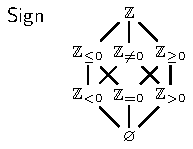
\includegraphics{sign-domain.pdf}
		\qquad\qquad
		% \begin{tikzpicture}[scale=0.7,shorten >=-2pt, shorten <=-2pt]
		% 	\draw (-1,-1) node[name=1] {\footnotesize$\varnothing$};
		% 	\draw (-2,0.2) node[name=2] {\footnotesize$\setZ_{<0}$};
		% 	\draw (-1,0.2) node[name=3] {\footnotesize$\setZ_{=0}$};
		% 	\draw (0,-0.3) node[name=9] {\footnotesize$\setZ_{=1}$};
		% 	\draw (0,0.6) node[name=4] {\footnotesize$\setZ_{>0}$};
		% 	\draw (-2,1.8) node[name=5] {\footnotesize$\setZ_{\leq 0}$};
		% 	\draw (-1,1.8) node[name=8] {\footnotesize$\setZ_{\neq 0}$};
		% 	\draw (-0,1.8) node[name=6] {\footnotesize$\setZ_{\geq 0}$};
		% 	\draw (-1,3) node[name=7] {\footnotesize$\setZ$};
		% 	\draw (-3,2.9) node[name=n] {{\normalsize $\Sign_1$}};
		%
		%
		% 	\draw[semithick] (1) -- (2);
		% 	\draw[semithick] (1) -- (3);
		% 	\draw[semithick] (2) -- (5);
		% 	\draw[semithick] (2) -- (8);
		% 	\draw[semithick] (3) -- (5);
		% 	\draw[semithick] (3) -- (6);
		% 	\draw[semithick] (4) -- (6);
		% 	\draw[semithick] (4) -- (8);
		% 	\draw[semithick] (5) -- (7);
		% 	\draw[semithick] (6) -- (7);
		% 	\draw[semithick] (8) -- (7);
		% 	\draw[semithick] (1) -- (9);
		% 	\draw[semithick] (9) -- (4);
		% \end{tikzpicture}
		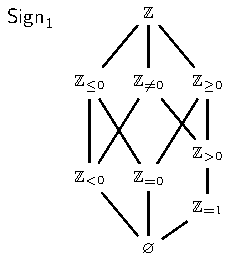
\includegraphics{sign1-domain.pdf}
	\end{center}

	For the command $\regr \eqdef \code{x := x - 1}$ and the concrete point $P = \{ 1 \}$ we have
	\[
	\Sign \denot{\regr}^{\Sign_{1}} \Sign_1(P) = \Sign \denot{\regr}^{\Sign_{1}} (\setZ_{= 1}) = \setZ_{= 0}
	\]
	but
	\[
	\Sign \denot{\regr}^{\Sign_1} \Sign(P) = \Sign \denot{\regr}^{\Sign_1} (\setZ_{> 0}) = \setZ_{\ge 0} .
	\]
\end{example}

Despite being necessary, the hypothesis of rule \lclrule{refine\mbox{-}ext} cannot be checked algorithmically because, in general, the bca $\denot{\regr}^{A'}$ of a composite command $\regr$ is not computable. To mitigate this issue, we present in Figure~\ref{fig:lcla:rules-refine-derived} two derived rules whose premises imply the premises of \lclrule{refine\mbox{-}ext}, thus ensuring extensional soundness via Theorem~\ref{th:lcla:soundness-rule-refine}.

\begin{figure*}[t]
	\begin{framed}
		\[
		\infer[\lclrule{refine\mbox{-}int}]
		{\lcl{A}{P}{\regr}{Q}}
		{\lcl{A'}{P}{\regr}{Q} \quad A' \preceq A \quad A \denot{\regr}^{\sharp}_{A'} A(P) = A(Q) }
		\]

		\[
		\infer[\lclrule{refine\mbox{-}pre}]
		{\lcl{A}{P}{\regr}{Q}}
		{\lcl{A'}{P}{\regr}{Q} \quad A' \preceq A \quad A'(P) = A(P) }
		\]
	\end{framed}
	\vspace{-1ex}
	\caption{Derived refinement rules for $\LCLA$.}\label{fig:lcla:rules-refine-derived}
\end{figure*}

The first rule we present replaces the requirement on the extensional bca $\denot{\regr}^{A'}$ with requirements on the intensional compositional abstraction $\denot{\regr}^{\sharp}_{A'}$ computed in $A'$. For this reason, we call this rule \lclrule{refine\mbox{-}int}.

The second derived rule we propose is simpler than \lclrule{refine\mbox{-}ext}: it just requires the abstractions $A(P)$ and $A'(P)$ to coincide, with no reference to the regular command $\regr$ nor to the postcondition $Q$. Since the premise is only on the precondition $P$, we call this rule \lclrule{refine\mbox{-}pre}.

\begin{prop}\label{th:lcla:refine-derived-sound}
	Both rules \lclrule{refine\mbox{-}int} and \lclrule{refine\mbox{-}pre} in Figure~\ref{fig:lcla:rules-refine-derived} are extensionally sound.
\end{prop}
\begin{proof}[Proof sketch]
	We show that the hypotheses of both rules imply those of \lclrule{refine\mbox{-}ext}. Since the first two hypotheses $\lcl{A'}{P}{\regr}{Q}$ and $A' \preceq A$ are shared among the rules, we only have to show that $\alpha \gamma' \denot{\regr}^{A'} \alpha' A(P) = \alpha(Q)$. The details are in Appendix~\ref{ch:app:lcla}.

	Because the hypotheses of \lclrule{refine\mbox{-}int} and \lclrule{refine\mbox{-}pre} implies those of \lclrule{refine\mbox{-}ext}, whenever we can apply the former we can also apply the latter, so that Theorem~\ref{th:lcla:soundness-rule-refine} ensures extensional soundness.
\end{proof}

It is worth noting that the condition in \lclrule{refine\mbox{-}int} on the compositional abstraction $\denot{\regr}^{\sharp}_{A'}$ can easily be checked by the analyser, possibly alongside the analysis of $\regr$ with LCL or using a stand-alone abstract interpreter.
Moreover, this rule is as powerful as the original \lclrule{refine\mbox{-}ext} because it enjoys a logical completeness result akin to Theorem~\ref{th:lcla:refinement-rule-completeness}.
\begin{theorem}[Logical completeness of \lclrule{refine\mbox{-}int}]\label{th:lcla:refine-int-completeness}
	Consider the proof system of Figure~\ref{fig:sota:lcla-rules} with the addition of rules \lclrule{refine\mbox{-}int} and \lclrule{limit}. If $Q \le \denot{\regr} P$ and $\denot{\regr}^A \alpha(P) = \alpha(Q)$ then $\lcl{A}{P}{\regr}{Q}$.
\end{theorem}
\begin{proof}
	The proof is the same as Theorem~\ref{th:lcla:refinement-rule-completeness}, the only difference being that to apply \lclrule{refine\mbox{-}int} we need to show $A \denot{\regr}^{\sharp}_{C} A(P) = A(\denot{\regr} P)$ instead of $A \denot{\regr}^{C} A(P) = A(\denot{\regr} P)$. However, since in the concrete domain $\denot{\regr}^{\sharp}_{C} = \denot{\regr}^{C} = \denot{\regr}$ the proof still holds.
\end{proof}

Just like logical completeness of \lclrule{refine\mbox{-}ext}, this result implies the existence of a refinement $A'$ (possibly the concrete domain) in which it is possible to carry out the proof.

Rule \lclrule{refine\mbox{-}pre} only requires a simple check at the application site instead of an expensive analysis of the program $\regr$, so it can be preferable in practice.
We present an example to highlight the advantages of this rule (as well as \lclrule{refine\mbox{-}int}), which allows us to use different domains in the proof derivation of different parts of the program.

\begin{example}[The use of \lclrule{refine\mbox{-}pre}]\label{ex:lcla:refine-pre-usefulness}
	Consider the two program fragments
	\begin{align*}
		\regr_1 & \eqdef \code{(y != 0)?; y := abs(y)}                                       \\
		\regr_2 & \eqdef \code{x := y; while (x > 1) \{ y := y - 1; x := x - 1 \}}           \\
		        & = \code{x := y; ((x > 1)?; y := y - 1; x := x - 1)$^{\kstar}$; (x <= 1)? }
	\end{align*}
	and the program $\regr \eqdef \regr_1; \regr_2$. Here \code{abs} is a function to compute the absolute value, and we assume, for the sake of simplicity, that the analyser knows its best abstraction. Consider the concrete domain $\pow(\setZ^2)$ where a pair $(n, m)$ denote a state $\code{x} = n$, $\code{y} = m$, and the initial state $P = (\code{y} \in [-100; 100])$, a logical description of the concrete points $\{ (n, m) \svert m \in [-100; 100] \} \in \pow(\setZ^2)$.
	The bca $\denot{\regr}^{\Int}$ in the abstract domain of intervals is locally complete on $P$ (since $P$ is expressible in $\Int$), but the compositional abstraction $\denot{\regr}^{\sharp}_{\Int}$ is not:
	\begin{align*}
		\denot{\regr}^{\Int} \alpha(P) & = \Int (\denot{\regr_2} \denot{\regr_1} (\{ (n, m) \svert m \in [-100; 100] \})) \\
		                               & = \Int (\denot{\regr_2} (\{ (n, m) \svert m \in [1; 100] \}))                    \\
		                               & = \Int (\{ (1, 1) \})                                                            \\
		                               & = ([1; 1] \times [1; 1]) ,
	\end{align*}
	while
	\begin{align*}
		\denot{\regr}^{\sharp}_{\Int} \alpha(P) & = \denot{\regr_2}^{\sharp}_{\Int} \denot{\regr_1}^{\sharp}_{\Int} ([-\infty; +\infty] \times [-100; 100])   \\
		                                        & = \denot{\regr_2}^{\sharp}_{\Int} \denot{\code{y := abs(y)}}^{\Int} ([-\infty; +\infty] \times [-100; 100]) \\
		                                        & = \denot{\regr_2}^{\sharp}_{\Int} ([-\infty; +\infty] \times [0; 100])                                      \\
		                                        & = ([1; 1] \times [0; 100]) \neq ([1; 1] \times [1; 1]) .
	\end{align*}
	The issues are twofold.
	First, the analysis of $\regr_1$ in $\Int$ is incomplete, so we need a more concrete domain. For instance, we can select $\Int_{\neq 0}$, the Moore closure of $\Int$ with the addition of the element $\setZ_{\neq 0}$ representing the property of being nonzero. Intuitively, $\Int_{\neq 0}$ contains all intervals, possibly having a ``hole" in $0$. Formally
	\[
	\Int_{\neq 0} = \Int \cup \{ I_{\neq 0} \svert I \in \Int \}
	\]
	with $\gamma'(I_{\neq 0 }) = \gamma(I) \setminus \{ 0 \}$.

	While there is no need for a relational domain to analyse $\regr_1$ since  variable \code{x} is never mentioned in it,
	the analysis of $\regr_2$ requires a relational domain to track the information that the value of variable \code{x} is equal to the value of variable \code{y}.
	This suggests to use the octagons domain $\Oct$~\cite{Mine06} to analyse $\regr_2$. It is worth noting that the abstract domain $\Oct$ would not be able to perform a locally complete analysis of $\regr_1$ for the same reasons that the domain $\Int$ could not.

	However, rule \lclrule{refine\mbox{-}pre} allows us to combine these different proof derivations. Since the program state between $\regr_1$ and $\regr_2$ can be precisely represented in $\Int$, we use this domain as a baseline and refine it to $\Int_{\neq 0}$ and to $\Oct$ for the two parts, respectively.

	Let $R = (\code{y} \in \{ 1; 2; 100 \})$ that is an under\hyp{}approximation of the concrete state in between $\regr_1$ and $\regr_2$ with the same abstraction in $\Int$, so the triple $\lcl{\Int}{P}{\regr_1}{R}$ is valid. Note that the concrete point $2$ was added to $R$ in order to have local completeness for \code{(x > 1)?} in $\regr_2$. However, this triple cannot be proved in $\Int$ because $\denot{\regr_1}^{\sharp}_{\Int}$ is not locally complete on $P$, so we resort to \lclrule{refine\mbox{-}pre} to change the domain to $\Int_{\neq 0}$.
	In the derivation below, we let $R_1 = (\code{y} \in [-100; 100] \land \code{y} \neq 0)$ and we omit for simplicity the additional hypothesis of \lclrule{relax}:
	\[
	\infer[(\mathsf{seq})]
	{\lcl{\Int_{\neq 0}}{P}{\regr_1}{R}
		%					\qquad \Int_{\neq 0} \preceq \Int \qquad \Int(P) = \Int_{\neq 0}(P)
	}
	{
		\infer[(\mathsf{transfer})]
		{\lcl{\Int_{\neq 0}}{P}{\code{y != 0?}}{R_1}}{ \complete{\Int_{\neq 0}}{P}{\denot{\code{y != 0?}}} }
		&
		\infer[(\mathsf{relax})]
		{\lcl{\Int_{\neq 0}}{R_1}{\code{y := abs(y)}}{R}}
		{\infer[(\mathsf{transfer})]
			{\lcl{\Int_{\neq 0}}{R_1}{\code{y := abs(y)}}{\code{y} \in [1; 100]}}{ \complete{\Int_{\neq 0}}{R_1}{\denot{\code{y := abs(y)}}} }
		}
	}
	\]

	Again $\denot{\regr_2}$ is locally complete on $R$ in $\Int$, but the compositional analysis $\denot{\regr_2}^{\sharp}_{\Int}$ is not. Hence to perform the derivation we resort to \lclrule{refine\mbox{-}pre} to introduce relational information in the abstract domain, using $\Oct$ instead of $\Int$. Let $Q = (\code{x} = 1 \land \code{y} = 1)$, that is the concrete output of the program, so that we can prove $\lcl{\Int}{R}{\regr_2}{Q}$.
	The derivation of this triple is in Appendix~\ref{ch:app:lcla}, Figure~\ref{fig:app:ex-refine-pre-derivation-2}. However, the proof is just a straightforward application of rules \lclrule{seq}, \lclrule{iterate} and \lclrule{transfer}.

	With those two derivation, we can prove the triple $\lcl{\Int}{P}{\regr}{Q}$ using \lclrule{refine\mbox{-}pre}:
	\[
	\infer[(\mathsf{seq})]
	{\lcl{\Int}{P}{\regr}{Q}}
	{
		\infer[(\mathsf{refine\mbox{-}pre})]
		{\lcl{\Int}{P}{\regr_1}{R}}
		{\lcl{\Int_{\neq 0}}{P}{\regr_1}{R}}
		&
		\infer[(\mathsf{refine\mbox{-}pre})]
		{\lcl{\Int}{R}{\regr_2}{Q}}
		{\lcl{\Oct}{R}{\regr_2}{Q}}
	}
	\]
	For space constraints, we write here the additional hypotheses of the rules. For the first application, $\Int_{\neq 0} \preceq \Int$ and $\Int_{\neq 0}(P) = P = \Int(P)$. For the second, $\Oct \preceq \Int$ and $\Int(R) = (\code{y} \in [1; 100]) = \Oct(R)$.

	It is worth noting that, in this example, all applications of \lclrule{refine\mbox{-}pre} can be replaced by \lclrule{refine\mbox{-}int}. This means that also the latter is able to exploit $\Int_{\neq 0}$ and $\Oct$ to prove the triple in the very same way, but its application requires more expensive abstract analyses than the simple checks of \lclrule{refine\mbox{-}pre}.
\end{example}

While \lclrule{refine\mbox{-}pre} is simpler than \lclrule{refine\mbox{-}ext} and \lclrule{refine\mbox{-}int}, it is also weaker in both a theoretical and practical sense. On the one hand, $\LCLA$ extended with this rule does not admit a logical completeness result; on the other hand, there are situations in which, even though \lclrule{refine\mbox{-}pre} allows a derivation, \lclrule{refine\mbox{-}int} is more effective. We show these two points by examples.
For the first, we propose a valid triple that $\LCLA$ extended with \lclrule{refine\mbox{-}pre} cannot prove.

\begin{example}[Logical incompleteness of \lclrule{refine\mbox{-}pre}]\label{ex:lcla:refine-pre-incomplete}
	Consider the program fragments\footnote{Note that $\regr_w$ is equivalent to the regular command $\code{false?}$.}
	\begin{align*}
		\regr_1 & \eqdef \code{x := x + 2}              \\
		\regr_w & \eqdef \code{while (true) \{ skip \}} \\
		\regr   & \eqdef \regr_1 \code{; }\regr_w
	\end{align*}
	the concrete domain $\pow(\setZ)$, the abstract domains $\Int_{\neq 0}$ (see Example~\ref{ex:lcla:refine-pre-usefulness}) and the initial state $P = \{ -4, 0 \}$.
	Then $\lclvalid{\Int_{\neq 0}}{P}{\regr}{\emptyset}$ but this triple cannot be proved in $\LCLA$ extended with \lclrule{refine\mbox{-}pre}.

	To show that the triple is (intensionally) valid, we observe that
	\[
	\denot{\regr}^{\sharp}_{\Int_{\neq 0}} \alpha(P) = \denot{\regr_w}^{\sharp}_{\Int_{\neq 0}} \denot{\regr_1}^{\sharp}_{\Int_{\neq 0}} \alpha(P) = \bot
	\]
	because $\regr_w$ always diverges, so $\denot{\regr_w}^{\sharp}_{\Int_{\neq 0}}$ too is the function that always diverge (in the abstract). Therefore,
	\[
	\denot{\regr}^{\sharp}_{\Int_{\neq 0}} \alpha(P) = \alpha(\denot{\regr} P) = \alpha(\emptyset) = \bot .
	\]
	To show that the triple is not provable in $\LCLA$ extended with \lclrule{refine\mbox{-}pre}, we rely on two observations.

	The first is that all strict subset $P' \subset P$ are such that $\Int_{\neq 0}(P') \subset P$, and the same property holds for all refinements $A' \preceq \Int_{\neq 0}$. To see this, take $P' \subset P$: there are only three such $P'$, and for all of them $\Int_{\neq 0}(P') = P' \subset P$. Moreover, $A' \preceq \Int_{\neq 0}$ means that $A'(P') \subseteq \Int_{\neq 0}(P')$, so
	\[
	A'(P') \subseteq \Int_{\neq 0}(P') = P' \subset P .
	\]
	This property is important because it means that we cannot apply \lclrule{relax} to change $P$: to do it, we would need a $P' \subset P$ such that $P \subseteq A'(P')$.

	The second is that $\denot{\regr_1}$ is not locally complete on $P$ in $\Int_{\neq 0}$ or any of its refinements $A' \preceq \Int_{\neq 0}$ such that $A'(P) = \Int_{\neq 0}(P)$:
	\begin{align*}
		A'(\denot{\regr_1} P) & \subseteq \Int_{\neq 0}(\denot{\regr_1} P)      \\
		                      & = \{ -2, -1, 1, 2 \}                            \\
		                      & \subset \{ -2, -1, 0, 1, 2 \}                   \\
		                      & \subseteq A'(\{ -2, -1, 0, 1, 2 \})             \\
		                      & = A'(\denot{\regr_1} (\{ -4, -3, -2, -1, 0 \})) \\
		                      & = A'(\denot{\regr_1} (\Int_{\neq 0}(P)))        \\
		                      & = A'(\denot{\regr_1} A'(P))
	\end{align*}

	Now suppose to have a derivation of $\lcl{\Int_{\neq 0}}{P}{\regr}{\emptyset}$. This proof must use \lclrule{seq} to handle the sequential composition $\regr_1 \code{; }\regr_w$, so it needs a triple for $\regr_1$. By the first observation above, any use of \lclrule{relax} cannot change the precondition of this triple, even if we resort first to \lclrule{refine\mbox{-}pre} to refine the domain. Thus we must have a triple $\lcl{A'}{P}{\regr_1}{R}$ for some $R$ and $A' \preceq \Int_{\neq 0}$ satisfying $A'(P) = \Int_{\neq 0}(P)$. However, by soundness, any such triple would imply local completeness of $\denot{\regr_1}$ on $P$ in $A'$, which is a contradiction by the second observation above.
\end{example}

Another example of a sound triple which is not provable using \lclrule{refine\mbox{-}pre}, which does not rely on divergence, is in Appendix~\ref{ch:app:lcla}, Example~\ref{ex:app:refine-pre-incomplete-2-appendix}.
A corollary of these examples (and more in general of logical incompleteness) is that there may not exist a refinement $A'$ to carry out the proof using \lclrule{refine\mbox{-}pre}.
Another consequence of this incompleteness result is the fact that, even when a command is locally complete in an abstract domain $A$, we may need to reason about properties that are not expressible in $A$ in order to prove it, as \lclrule{refine\mbox{-}pre} may not be sufficient.

We now present an example to illustrate that there are situations in which \lclrule{refine\mbox{-}int} is more practical than \lclrule{refine\mbox{-}pre}, even though they are both able to prove the same triple.
\begin{example}
	Consider the two program fragments
	\begin{align*}
		\regr_1 & \eqdef \code{(y != 0)?; x := y; y := abs(y)}                     \\
		\regr_2 & \eqdef \code{x := y; while (x > 1) \{ y := y - 1; x := x - 1 \}}
	\end{align*}
	and the program $\regr \eqdef \regr_1; \regr_2$. Consider also the initial state $P = \code{y} \in [-100; 100]$.

	This example is a variation of Example~\ref{ex:lcla:refine-pre-usefulness}: the difference is the introduction of the relational dependency \code{x := y} in $\regr_1$, that is partially stored in the postcondition $R$ of $\regr_1$. Because of this, $\Oct(R)$ and $\Int(R)$ are different, so we cannot apply \lclrule{refine\mbox{-}pre} to prove $\lcl{}{R}{\regr_2}{Q}$ for some $Q$.

	%	We keep $\regr$ deliberately simple, but an actual program could do something between $\regr_1$ and $\regr_2$ with the value in \code{x}.

	Following Example~\ref{ex:lcla:refine-pre-usefulness}, the domain $\Int_{\neq 0}$ is able to infer on $\regr_1$ a subset $R$ of the strongest postcondition $\code{y} \in [1; 100] \land \code{y} = \text{abs}(\code{x})$ with the same abstraction $\Int_{\neq 0}(R) = [-100; 100]_{\neq 0} \times [1; 100]$. However, for any such $R$ we cannot use \lclrule{refine\mbox{-}pre} to prove the triple $\lcl{\Int}{R}{\regr_2}{\code{x} = 1 \land \code{y} = 1}$ via $\Oct$ because $\Int(R) = \code{x} \in [-100; 100] \land \code{y} \in [1; 100]$ while $\Oct(R) = 1 \le \code{y} \le 100 \land -\code{y} \le \code{x} \le \code{y}$. More in general, any subset of the strongest postcondition contains the relational information $\code{y} = \text{abs}(\code{x})$, so relational domains like octagons and polyhedra \cite{CH78} do not have the same abstraction as the non-relational $\Int$, preventing the use of \lclrule{refine\mbox{-}pre}. However, we can apply \lclrule{refine\mbox{-}int}: considering $R = (\code{y} \in \{1; 2; 100\} \land \code{y} = \text{abs}(\code{x}) )$, $Q = (\code{x} = 1 \land \code{y} = 1)$ and $\regr_w \eqdef \code{while (x > 1) \{ y := y - 1; x := x - 1 \}}$, we have
	\begin{align*}
		\Int \denot{\regr_2}^{\sharp}_{\Oct} \Int(R) & = \Int \denot{\regr_2}^{\sharp}_{\Oct} (\code{x} \in [-100; 100] \land \code{y} \in [1; 100])                                       \\
		                                             & = \Int \denot{\regr_w}^{\sharp}_{\Oct} \denot{\code{x := y}}^{\sharp}_{\Oct} (\code{x} \in [-100; 100] \land \code{y} \in [1; 100]) \\
		                                             & = \Int \denot{\regr_w}^{\sharp}_{\Oct} (1 \le \code{y} \le 100, \code{y} = \code{x})                                                \\
		                                             & = \Int(\code{x} = 1 \land \code{y} = 1)                                                                                             \\
		                                             & = \Int(Q) .
	\end{align*}

	In this example, rule \lclrule{refine\mbox{-}pre} can be applied to prove the triple, but it requires to have relational information from the assignment \code{x := y} in $\regr_1$, hence forcing the use of a relational domain (e.g. the reduced product~\cite{CC79} of $\Oct$ and $\Int_{\neq 0}$) for the whole $\regr$, making the analysis more expensive.
\end{example}

\subsection{Choosing the refinement}\label{sec:lcla:choose-refinement}
Thanks to the three new rules \lclrule{refine\mbox{-}ext}, \lclrule{refine\mbox{-}int} and \lclrule{refine\mbox{-}pre} we can now combine different domains in the same derivation.
However, in order to obtain an algorithm that automatises the search of a provable $\LCLA$ triple we are left with the problem of the selection of the right refinement to use each time. A crucial point to the applicability of refine rules is a strategy to find the most convenient refined abstract domain. While we have not addressed this problem yet, we believe there are some interesting starting points in the literature.

In previous sections, we settled the question from a theoretical point of view. Logical completeness results for \lclrule{refine\mbox{-}ext} (Theorem~\ref{th:lcla:refinement-rule-completeness}) and \lclrule{refine\mbox{-}int} (Theorem~\ref{th:lcla:refine-int-completeness}) implies the existence of a domain in which it is possible to complete the proof (if this were not the case, then the proof could not be completed in any domain, contradicting logical completeness). However, the proofs of those theorems exhibit the concrete domain $C$ as an example, which is unfeasible in general. Dually, as \lclrule{refine\mbox{-}pre} is logically incomplete (Example~\ref{ex:lcla:refine-pre-incomplete}), there are triples that cannot be proved in any domain with it.

As more practical alternatives, we envisage some possibilities.
First, we are studying relationships with counterexample\hyp{}guided abstraction refinement (CEGAR) \cite{CGJLV00}, which is a technique that exploits refinement in the context of abstract model checking. However, CEGAR and our approach seem complementary. On the one hand, our refinement rules allow a dynamic change of domain, during the analysis and only for a part of it, while CEGAR performs a static refinement and then a new analysis of the whole transition system in the new, more precise domain. On the other hand, our rules lack an instantiation technique, while for CEGAR there are effective algorithms available to pick a suitable refinement.

Second, local completeness shell \cite{BGGR22} were proposed as an analogous of (global) completeness shell \cite{GRS00}. In the article, the authors proposed to use local completeness shells to perform abstract interpretation repair, a technique to refine the abstract domain depending on the program to analyse, just like CEGAR does for abstract model checking. Abstract interpretation repair works well with $\LCLA$, and could be a way to decide the best refinement for one of our rules in presence of a failed local completeness proof obligation. The advantage of combining repair with our new rules is given by the possibility of discarding the refined domain just after its use in a subderivation instead of using it to carry out the whole derivation. Investigations in this direction is ongoing.

Another related approach, which shares some common ground with CEGAR, is Lazy (Predicate) Abstraction \cite{HJMS02,McMillan06}. Both ours and this approach exploits different abstract domains for different parts of the proof, refining it as needed. The key difference is that Lazy Abstraction unwinds the control flow graph of the program (with techniques to handle loops) while we work inductively on the syntax. This means that, when Lazy Abstraction refines a domain, it must use it from that point onward (unless it finds a loop invariant). On the other hand, our method can change abstract domain even for different parts of sequential code. However, the technique used in Lazy Abstraction (basically to trace a counterexample back with a theorem prover until it is either found to be spurious or proved to be true) could be applicable to $\LCLA$: a failed local completeness proof obligation in \lclrule{transfer} can be traced back with a theorem prover and the failed proof can be used to understand how to refine the abstract domain.

\section{Locally complete simplification}
We now turn our attention to \emph{simplification} of the abstract domain in the $\LCLA$ proof system. It is known that (global) completeness can be achieved both by refining and by simplifying the abstract domain (these construction are called completeness shell and core, respectively~\cite{GRS00}). Therefore, we do the same for local completeness.
We propose the rule \lclrule{simplify}, in Figure~\ref{fig:lcla:rule-simplify}. This is a dual of \lclrule{refine\mbox{-}pre}: while the latter requires $A'$ to be a refinement of $A$ with the same abstraction on the precondition $P$, the former requires $A'$ to be a simplification of $A$ with the same abstraction on the postcondition $Q$. We remark that this rule is independent of the refinement ones: it can be added to $\LCLA$ both with and without any of the refinement rules.

The proposed rule \lclrule{simplify} is sound, but differently than the refinement rules, it is so \emph{intensionally}:

\begin{figure*}[t]
	\begin{framed}
		\[
		\infer[\lclrule{simplify}]
		{\lcl{A}{P}{\regr}{Q}}
		{\lcl{A'}{P}{\regr}{Q} & A' \succeq A & A'(Q) = A(Q)}
		\]
	\end{framed}
	\vspace{-1ex}
	\caption{Rule \lclrule{simplify} for $\LCLA$.}\label{fig:lcla:rule-simplify}
\end{figure*}

\begin{theorem}[Intensional soundness of rule simplify]\label{th:lcla:soundness-rule-simpl}
	The proof system in Figure~\ref{fig:sota:lcla-rules} with the addition of rule \lclrule{simplify} from Figure~\ref{fig:lcla:rule-simplify} is intensionally sound.
\end{theorem}
\begin{proof}[Proof sketch]
	Since the proof of Theorem~\ref{th:sota:lcl-soundness} in~\cite{BGGR21} is by rule induction, we extend its proof with a new inductive case. The full details are in Appendix~\ref{ch:app:lcla}.
\end{proof}

This result is somewhat surprising: for completeness, refinement and simplification have the same power; instead, for local completeness, the former appears to be stronger than the latter.

Even though rule \lclrule{simplify} does not allow the proof system to prove triples which are not intensionally sound, it still allows to prove more triples, as shown in the following example.

\begin{example}\label{ex:lcla:simplify-stronger}
	This example builds on the previous Example~\ref{ex:lcla:refine-pre-incomplete}.
	Consider the same program fragments $\regr_1$, $\regr_w$ and $\regr$, concrete domain $\pow(\setZ)$, abstract domain $\Int_{\neq 0}$, initial state $P = \{ -5, 0 \}$ and final state $\emptyset$.
	We already showed that the triple $\lcl{\Int_{\neq 0}}{P}{\regr}{\emptyset}$ cannot be proved using $\LCLA$ (extended with \lclrule{refine\mbox{-}pre}) in Example~\ref{ex:lcla:refine-pre-incomplete}. Hence, we only need to show that it is provable using \lclrule{simplify}.

	Consider the simplified domain $\Div = \{ \bot, \top \} \succeq \Int_{\neq 0}$.
	The domain $\Div$ separates the empty set from any other set, and can be used for divergence analysis.
	$\denot{\regr_1}$ is locally complete on $P$ in $\Div$:
	\begin{equation*}
		\Div(\denot{\regr_1}(P)) = \top = \Div(\denot{\regr_1}(\top)) = \Div(\denot{\regr_1}(\Div(P)))
	\end{equation*}
	This means we can prove the triple $\lcl{\Div}{P}{\regr_1}{ \denot{\regr_1}(P) }$ by just applying \lclrule{transfer}. Moreover, $\denot{\regr_w}$ is globally complete since its output is always $\emptyset$. With these two observations, we can derive the triple $\lcl{\Int_{\neq 0}}{P}{\regr}{\emptyset}$ using \lclrule{simplify} with the following proof tree:
	\[
	\infer[(\mathsf{simplify})]
	{ \lcl{\Int_{\neq 0}}{P}{\regr}{\emptyset} }
	{
		\infer[(\mathsf{seq})]
		{
			\Div \succeq \Int_{\neq 0}
			\qquad \lcl{\Div}{P}{\regr}{\emptyset}
			\qquad \Int_{\neq 0}(\emptyset) = \emptyset = \Div(\emptyset)
		}
		{
			\infer[(\mathsf{transfer})]
			{ \lcl{\Div}{P}{\regr_1}{\denot{\regr_1}(P)} }
			{ \complete{\Div}{P}{\denot{\regr_1}} }
			&
			\infer[(\mathsf{transfer})]
			{ \lcl{\Div}{\denot{\regr_1}(P)}{\regr_w}{\emptyset} }
			{ \complete{\Div}{\denot{\regr_1}(P)}{\denot{\regr_w}} }
		}
	}
	\]
\end{example}

Intuitively, in the previous example the incompleteness is caused by the precision of $\Int_{\neq 0}$ on the output of $\regr_1$. However, this precision is not needed because the details of the intermediate state are discarded by $\regr_w$. The simpler domain $\Div$ is able to discard such precision, thus proving local completeness of the composite command.

In this example, we showed that $\lcl{\Int_{\neq 0}}{P}{\regr}{\emptyset}$ can be proved in $\LCLA$ extended with \lclrule{simplify}, but by Example~\ref{ex:lcla:refine-pre-incomplete} we know it is not provable by \lclrule{refine\mbox{-}pre}. We remark that the opposite is true as well: $\LCLA$ extended with \lclrule{refine\mbox{-}pre} can prove extensionally valid triples (cf. Example~\ref{ex:lcla:refine-pre-usefulness}) that it cannot prove when extended with \lclrule{simplify}, because the latter is bound by intensional soundness. Together, these two facts means that \lclrule{refine\mbox{-}pre} and \lclrule{simplify} extend the logic in two incomparable ways. If we instead include \lclrule{refine\mbox{-}int}, we know by logical completeness (Theorem~\ref{th:lcla:refine-int-completeness}) that it can prove all (extensionally) valid triples, including all those provable with \lclrule{simplify}.

However, even though $\LCLA$ extended with \lclrule{simplify} can prove more triples, it is logically incomplete:

\begin{theorem}[Intrinsic incompleteness]\label{th:lcla:intrinsic-incompl-simplify}
	Consider the concrete domain of stores $C = \pow(\Sigma)$. Assume $\Reg$ is a Turing complete language, and $A \in \Abs(C)$ is not trivial. Then there exists $P, Q \in C$ and $\regr \in \Reg$ such that $Q \le \denot{\regr} P$, $\denot{\regr}^{\sharp}_A \alpha(P) = \alpha(Q)$ but the triple $\lcl{A}{P}{\regr}{Q}$ is not provable in $\LCLA$ extended with \lclrule{simplify}.
\end{theorem}
\begin{proof}[Proof sketch]
	The proof follows closely that of intrinsic incompleteness of $\LCLA$ \cite[Theorem~5.12]{BGGR21} and is reported in Appendix~\ref{ch:app:lcla}.
\end{proof}

This theorem shows that the strength of rule \lclrule{simplify} on the logical level is quite thin.
However, this rule could be extremely helpful in practice because it allows to perform part of the analysis in a simpler and possibly much more efficient domain.
For instance, consider variable partitioning, a kind of domain simplification. In a series of papers, Singh et al.~\cite{SPV15,SPV17,SPV18} showed that it leads to great speedups in relational numerical abstract domains, such as octagons and polyhedra. Variable partitioning is a technique that divides variables in subsets such that relations only exists among variables in the same subset. This allows to perform many operations separately on different partitions, reducing the cost that is superlinear in the number of variables (eg. cubic for octagons, exponential for polyhedra). Moreover, partitions are chosen dynamically, so that (1) they change during the analysis and (2) they are guaranteed not to lose precision w.r.t. the non partitioned domain.
Let us consider the domain $\Poly$ of polyhedra as an example, but we remark these observations are general enough to be applied to many relational numerical domains.
Formally, given a set of variables $\Var$ and one of its partitions $\pi = \{ \mathcal{X}_1, \mathcal{X}_2, \dots, \mathcal{X}_m \}$, a polyhedron $P$ can be expressed in the partition $\pi$ if and only if, for all constraints $k$ of $P$ all variables involved in $k$ are in the same element $\mathcal{X}_i \in \pi$.
%From a theoretical point of view, variable partitioning is a \emph{simplification} of the abstract domain.
Given a variable partitioning $\pi$ we denote by $\Poly_{\pi}$ the abstract domain of polyhedra that can be expressed in the partition $\pi$. Clearly $\gamma(\Poly_{\pi}) \subseteq \gamma(\Poly)$, so that $\Poly \preceq \Poly_{\pi}$ for all $\pi$.
Since the partition is changed during the analysis, the abstract domain changes too. Rule \lclrule{refine\mbox{-}ext} cannot accommodate for this change. A domain coarser than all partitions correspond to the maximal partition, in which each variable is on its own, and is non relational: for $\Poly$ this domain is $\Int$. In general $\Int$ is not precise enough to prove the condition $A \denot{\regr}^{A'} A(P) = A(Q)$ (instantiated with $A = \Int$ and $A' = \Poly_{\pi}$ it becomes $\Int \denot{\regr}^{\Poly_{\pi}} \Int(P) = \Int(Q)$) at every partition change, since those occur during the analysis and must keep track of relational informations computed up to that point.
On the other hand, rule \lclrule{simplify} perform the ``global" analysis in $\Poly$, and simplify locally to $\Poly_{\pi}$ for the computation, taking advantage of the better performances in the simpler domain. Note that, since the partition is chosen in order not to lose precision w.r.t. the non partitioned domain $\Poly$, the condition $A'(Q) = A(Q)$ is satisfied. This means that variable partitioning can be plugged in $\LCLA$ with our rule \lclrule{simplify}, allowing it to benefit from all the performance increase. While it is intuitive that variable partitioning is sound since it is as precise as $\Poly$, our rule formally justify this claim.

\begin{example}
	Consider the program fragments
	\begin{align*}
		\regr_1 & \eqdef \code{x := y; y := y - 3; x := x - 4}                        \\
		\regr_2 & \eqdef \code{z := y; y := 0}                                        \\
		\regr_3 & \eqdef \code{w := z - x}                                            \\
		\regr   & \eqdef \regr_1; \regr_2; \regr_3                                    \\
		        & = \code{x := y; y := y - 3; x := x - 4; z := y; y := 0; w := z - x}
	\end{align*}
	and the initial state $P = -100 \le y \le 100$. At the end, the value for $\code{w}$ is always $1$. To prove it, the analysis must track the dependency between variables using a relational domain such as polyhedra. However, for the first three assignments (i.e., the fragment $\regr_1$) we do not need to track any dependency involving $\code{z}$ and $\code{w}$, and after the assignment \code{y := 0} in $\regr_2$ there is no dependency to track with $\code{y}$.

	Consider the final set of states
	\[
	Q \eqdef (y = 0 \land x \in \{ -104, 96 \} \land z = x + 1 \land w = 1)
	\]
	and partitions $\pi_1 = \{ \{ x , y \}, \{ z \}, \{ w \} \}$ and $\pi_2 = \{ \{ x, z \}, \{ y \}, \{ w \} \}$.
	A proof for the triple $\lcl{\Poly}{P}{\regr}{Q}$ can exploit \lclrule{simplify} to work in $\Poly_{\pi_1}$ and $\Poly_{\pi_2}$ for parts of the program, therefore simplifying the computation of the local completeness proof obligations for \lclrule{transfer}. Fixed $R_1 \eqdef (y \in \{ -103, 97 \} \land x = y - 1)$ and $R_2 \eqdef (x \in \{ -104, 96 \} \land y = 0 \land z = x + 1)$, the proof sketch looks like

	\[
	\infer[\lclrule{seq}]
	{\lcl{\Poly}{P}{\regr}{Q}}
	{
		\infer[\lclrule{simplify}]
		{\lcl{\Poly}{P}{\regr_1}{R_1}}
		{\infer{\lcl{\Poly_{\pi_1}}{P}{\regr_1}{R_1}}{\dots}}
		&
		\infer{\lcl{\Poly}{R_1}{\regr_2}{R_2}}{\dots}
		&
		\infer[\lclrule{simplify}]
		{\lcl{\Poly}{R_2}{\regr_3}{Q}}
		{\infer{\lcl{\Poly_{\pi_2}}{R_2}{\regr_3}{Q}}{\dots}}
	}
	\]

	Note that $\Poly(R_1) = \Poly_{\pi_1}(R_1)$ and $\Poly(Q) = \Poly_{\pi_2}(Q)$ because $R_1$ (resp. $Q$) only contains constraints between variables in the same partition of $\pi_1$ (resp. $\pi_2$).
\end{example}

Since \lclrule{simplify} is analogous to \lclrule{refine\mbox{-}pre}, a natural question is whether there exists one simplification rule similar to the stronger \lclrule{refine\mbox{-}ext}. We believe this is not the case.
A dual of \lclrule{refine\mbox{-}ext} for simplification should involve $\denot{\regr}^{A'}$, because the goal of the rule is to perform the analysis in $A'$. The only reasonable input to which we can apply $\denot{\regr}^{A'}$ is $\alpha'(P)$. Note that, since $A' \succeq A$, abstracting with $A$ before does not change the result: $\alpha' A(P) = \alpha'(P)$. The hypothesis $\lcl{A'}{P}{\regr}{Q}$ implies, by soundness, $\denot{\regr}^{A'} \alpha'(P) = \alpha'(Q)$. Moreover, for the rule to be sound its hypotheses must ensure that $\alpha(Q) = \alpha(\denot{\regr} P) = \denot{\regr}^{A} \alpha(P)$, so any condition involving $\denot{\regr}^{A'} \alpha'(P)$ and any of those three is equivalent to $A'(Q) = A(Q)$.
Based on this argument, we don't expect a weaker condition (that is, a more general rule) for simplification to exist.

\section{Exploiting convexity}
$\LCLA$ requires the existence of a best correct abstraction $\alpha : C \rightarrow A$, but there are domains for which only the concretisation map $\gamma$ is defined (e.g., for polyhedra). If this is the case, $\LCLA$ is not applicable because we cannot even write the (local) completeness equation $A f(P) = A f A(P)$.
However, local completeness enjoys abstract convexity (Lemma~\ref{lmm:sota:abstract-convexity}). This suggests that, even if a concrete point $X$ cannot be abstracted, we can use a different point $P$ that can be abstracted such that $P \le X \le A(P)$. Intuitively, if $f$ is locally complete on $P$, abstract convexity implies that $f$ is locally complete on $x$, too. This idea is the basis of the development in this section.

Formally, we introduce an intermediate domain $L$ between $C$ and $A$ such that (1) there is a Galois connection between $L$ and $A$ and (2) we have a monotone concretisation function $\gamma_0 : L \rightarrow C$, as in the following diagram:
\[
C \xleftarrow{\gamma_0} L \mathrel{\substack{\gamma \\ \leftrightarrows \\ \alpha}} A
\]
Intuitively, we take $L$ as the set of all the assertions we can write as pre and postconditions of $\LCLA$ triples, and we limit this to be only a subset of $C$ for which there is an abstraction function $\alpha : L \rightarrow A$. For instance, if $A = \Poly$, we can take $L$ to be the set of finite unions of polyhedra, and limit the logic to only use those as pre and postconditions of triples, instead of any possible concrete state.
To apply $\LCLA$ using $L$ as the concrete domain, we fix an abstraction $\denot{\regr}_L : L \rightarrow L$ of $\denot{\regr}$. As it is standard in the absence of the abstraction function~\cite{CC92}, we require $\denot{\regr}_L$ to satisfy the soundness condition $\denot{\regr} \gamma_0 \le \gamma_0 \denot{\regr}_L$.
Since there is a Galois connection between $L$ and $A$, we can exploit the $\LCLA$ framework (and all of its extensions) using $L$ as the concrete domain and $\denot{\regr}_L$ as the concrete semantics. Then , to transfer the nice properties of $\LCLA$ from $L$ to $C$, we require the concrete point $X \in C$ to be in between the current assertion $P \in L$ and its abstraction $\alpha(P) \in A$. Formally, at any program point with concrete state $X$ and assertion $P$, we require that
\begin{equation*}\label{eqn:lcla:I}
	\gamma_0(P) \le X \le \gamma_0\gamma\alpha(P) \tag{I}
\end{equation*}
Please note that, if this invariant holds after the execution of a program $\regr$, then the Proofs of Verification (Corollary~\ref{th:sota:corollary-verification}) holds for the concrete value $X$.

However, in general this invariant is not preserved by program execution. Given a triple $\lcl{A}{P}{\regr}{Q}$ (w.r.t. the concrete domain $L$ and semantics $\denot{\regr}_L$) such that the concrete state before $\regr$ is $X$ satisfying~\eqref{eqn:lcla:I}, in general the corresponding invariant after the program $\gamma_0(Q) \le \denot{\regr} X \le \gamma_0\gamma\alpha(Q)$ does not hold. This is because $\denot{\regr} X$ may not be comparable with $\gamma_0 (\denot{\regr}_L P)$ even if $\denot{\regr}_L$ is sound. To solve this issue, we impose the additional condition of forward completeness~\cite{GQ01} of $\denot{\regr}_L$, but only on the single point $P$, namely
\[
\gamma_0(\denot{\regr}_L P) = \denot{\regr} \gamma_0(P) .
\]

Under this hypothesis, we show the following proposition:

\begin{prop}\label{prop:lcla:no-alpha-soundness}
	Assume that $\denot{\regr}_L$ is forward complete on $P$, that $\lclvalid{A}{P}{\regr}{Q}$ is valid taking $L$ as the concrete domain and that invariant~\eqref{eqn:lcla:I} holds.
	Then
	\[
	\gamma_0(Q) \le \denot{\regr} X \le \gamma_0\gamma\alpha(Q) \text{.}
	\]
\end{prop}
\begin{proof}
	We prove the two inequalities separately. We recall that $\denot{\regr}$ and $\gamma_0$ are monotone, and we use this fact implicitly in the chains of inequalities below.
	\begin{align*}
		\gamma_0 (Q) & \le \gamma_0 (\denot{\regr}_L P) & [\text{validity of }\lcl{A}{P}{\regr}{Q}\text{, pt. (1)}] \\
		             & = \denot{\regr} \gamma_0(P)      & [\text{forward completeness}]                             \\
		             & \le \denot{\regr} X              & [\gamma_0(P) \le X]
	\end{align*}
	and
	\begin{align*}
		\denot{\regr} X & \le \denot{\regr} \gamma_0 \gamma \alpha(P)         & [X \le \gamma_0 \gamma \alpha(P)]                         \\
		                & \le \gamma_0 (\denot{\regr}_L \gamma\alpha(P))      & [\text{soundness of }\denot{\regr}_L]                     \\
		                & \le \gamma_0 \gamma ((\denot{\regr}_L)^A \alpha(P)) & [\text{soundness of }(\denot{\regr}_L)^A]                 \\
		                & = \gamma_0 \gamma \alpha(Q)                         & [\text{validity of }\lcl{A}{P}{\regr}{Q}\text{, pt. (3)}]
	\end{align*}
\end{proof}

This lemma allows us to use $\LCLA$ even in the absence of a best abstraction function. However, to do so we need to identify a set $L$ of assertions which is concrete enough to be forward complete and abstract enough to have an abstraction function $\alpha: L \rightarrow A$.

Intuitively, the (local) forward completeness requirement $\gamma_0(\denot{\regr}_L P) = \denot{\regr} \gamma_0(P)$ implies that all the concrete state traversed are ``close enough'' to have an abstraction that a proof in $\LCLA$ yields useful information. In other words, the local forward completeness is a ``sanity check'' that the program did not traverse a concrete state for which the $\LCLA$ theory is not applicable, that are states $X$ for which there exists no $P \in L$ s.t. \eqref{eqn:lcla:I} holds. For instance, with the previous example of polyhedra and finite unions of polyhedra, any shape with a curved ``edge'' (e.g., a circle) does not satisfy the requirement \eqref{eqn:lcla:I}, and the local forward completeness condition ensures such states are not traversed.
\begin{example}
	Consider the concrete domain $\mathbb{R}^2$ of two real variables $\code{x}$ and $\code{y}$, the polyhedra domain $\Poly$ as $A$ and the set of finite unions of polyhedra $\Poly_{\cup}$ as $L$.
	Consider the program fragment
	\begin{align*}
		\regr_r & \eqdef \code{x := ($\sqrt{2}$ / $2$) * x - ($\sqrt{2}$ / $2$) * y; y := x + $\sqrt{2}$ * y}
	\end{align*}
	the program $\regr \eqdef \regr_r^\kstar$ and the set of states $X = -5 \le x \le 5 \land -5 \le y \le 5$, describing a square in the Cartesian plane. Please note that the program $\regr_r$ rotates the point $(x, y)$ in the Cartesian plane by $\pi / 4$ radiants, therefore applying $\regr_r$ to $X$ twice returns $X$. In particular, letting $X' \eqdef \denot{\regr_r} X$, this means that $\denot{\regr} X = X \cup X'$.

	Consider the initial assertion $P = \{ (5, 5), (-5, 5), (5, -5), (-5, -5) \}$, where a pair denote the value for variables $\code{x}$ and $\code{y}$, that is the union of four polyhedra, each containing a single point. It holds that $\gamma_0(P) \subseteq X = \gamma_0 (\Poly(P))$. We also define $P' = \{ (5 \sqrt{2}, 0), (- 5 \sqrt{2}, 0), (0, 5 \sqrt{2}), (0, -5 \sqrt{2}) \}$ and $Q = P \cup P'$.
	Using $\text{LCL}_{\Poly}$ over $L=\Poly_{\cup}$, we can first prove the two triples $\lcl{\Poly}{P}{\regr_r}{P'}$ and $\lcl{\Poly}{P \cup P'}{\regr_r}{Q}$ using \lclrule{seq} and \lclrule{transfer}. Then, we compose them using \lclrule{iterate} and \lclrule{req} to conclude:
	\[
	\infer[\lclrule{rec}]
	{\lcl{\Poly}{P}{\regr}{P \cup Q}}
	{
		\infer{\lcl{\Poly}{P}{\regr_r}{P'}}{\dots}
		&
		\infer[\lclrule{iterate}]
		{\lcl{\Poly}{P \cup P'}{\regr_r^\kstar}{Q}}
		{
			\infer{\lcl{\Poly}{P \cup P'}{\regr_r}{Q}}{\dots}
			&
			(P \cup P') \le \Poly(Q)
		}
	}
	\]

	This tells us that the triple $\lcl{\Poly}{P}{\regr}{P \cup Q}$ is valid relative to the semantics in $\Poly_{\cup}$. To transfer the same analysis to the concrete domain $\mathbb{R}^2$, we  check forward completeness. In this case, the check is trivial because the semantics of $\regr$ in $L$ on $P$, $P'$ and $Q$ is exactly the same as the concrete semantics on $\gamma_0(P)$, $\gamma_0(P')$ and $\gamma_0(Q)$.
	Note that this triple allows us to identify errors: given the specification Spec $= x \le 7$, we observe that $Q \nleq $ Spec. Since Spec is expressible in $\Poly$, this in turn highlights the error $(5 \sqrt{2}, 0) \in Q \setminus $Spec, which is a true alert because $(5 \sqrt{2}, 0) \in X \cup X'$.
\end{example}

\section{Backward analysis}

In principle, the theory of Abstract Interpretation does not rely on the analysis being forward. This suggests that LCL can be used for backward analysis, as discussed in~\cite[\S 5.3]{BGGR23}. However, they explored the use of \wlp{} as the reference backwards semantics, requiring the use of under\hyp{}approximation abstract domains, that are hard to exploit in practice (see Chapter~\ref{ch:uai}).
Instead, our key insight is that by using $\bwsem{\cdot}$ (see equation~\eqref{eq:sil:bwsem-definition}) the proof system can be turned over by duality for backward inference \emph{using classical, over-approximation abstract domains}.

\begin{figure*}
	\begin{align*}
		\bwsem{\expe}^{\sharp}_{A} a                    & \eqdef \bwsem{\expe}^{A} a = \alpha \bwsem{\expe} \gamma (a)                \\
		\bwsem{\regr_1 ; \regr_2}^{\sharp}_{A} a        & \eqdef \bwsem{\regr_2}^{\sharp}_{A} \bwsem{\regr_1}^{\sharp}_{A} (a)        \\
		\bwsem{\regr_1 \regplus \regr_2}^{\sharp}_{A} a & \eqdef \bwsem{\regr_1}^{\sharp}_{A} a \vee A \bwsem{\regr_2}^{\sharp}_{A} a \\
		\bwsem{\regr^\kstar}^{\sharp}_{A} a             & \eqdef \bigvee_{n \ge 0}  (\bwsem{\regr}^{\sharp}_{A})^n a
	\end{align*}
	\caption{Backward abstract semantics of regular commands.}
	\label{fig:lcla:regcom-abs-sem-bw}
\end{figure*}

We define inductively in Figure~\ref{fig:lcla:regcom-abs-sem-bw} the backward abstract semantics or regular commands. This definition is analogous to the forward one (Figure~\ref{fig:bg:regcom-abs-sem}). Thanks to Lemma~\ref{lmm:sil:bwsem-calculus} giving $\bwsem{\cdot}$ the same inductive definition as the forward semantics $\fwsem{\cdot}$, we can straightforwardly adapt Proposition~\ref{prop:bg:regcom-abs-sem-sound} to obtain that $\bwsem{\cdot}^{\sharp}_{A}$ is a sound abstraction of $\bwsem{\cdot}$.

\begin{figure*}[t]
	\centering
	\begin{framed}
		\resizebox{\textwidth}{!}{\(
			\begin{array}{l}
				\infer[\clclrule{transfer}]
				{\clcltriple{A}{\bwsem{\regc}Q}{\regc}{Q}}
				{\complete{A}{Q}{\bwsem{\regc}}}
				\quad
				\infer[\clclrule{relax}]
				{\clcltriple{A}{P}{\regr}{Q}}
				{P \le P' \le A(P)                         & \clcltriple{A}{P'}{\regr}{Q'}    & Q' \le Q \le A(Q')}
				\\[7.5pt]
				\infer[\clclrule{seq}]
				{\clcltriple{A}{P}{\regr_1;\regr_2}{Q}}
				{\clcltriple{A}{P}{\regr_1}{R}             & \clcltriple{A}{R}{\regr_2}{Q}}
				\hfill
				\infer[\clclrule{join}]
				{\clcltriple{A}{P_1 \lor P_2}{\regr_1 \regplus \regr_2}{Q}}
				{ \clcltriple{A}{P_1}{\regr_1}{Q}          & \clcltriple{A}{P_2}{\regr_2}{Q}}
				\\[7.5pt]
				\infer[\clclrule{rec}]
				{\clcltriple{A}{P}{\regr^\kstar}{Q}}
				{\clcltriple{A}{P}{\regr^\kstar}{R \lor Q} & \clcltriple{A}{R}{\regr}{Q}}
				\hfill
				\infer[\clclrule{iterate}]
				{\clcltriple{A}{P \lor Q}{\regr^\kstar}{Q}}
				{P \le A(Q)                                & \clcltriple{A}{P}{\regr}{Q}}
			\end{array}
			\)}
	\end{framed}
	\caption{The proof system for CLCL.}
	\label{fig:lcla:clcl-rules}
\end{figure*}

We can then define the proof system for Converse Local Completeness Logic~(CLCL) in Figure~\ref{fig:lcla:clcl-rules} by just swapping the roles of pre and post in the LCL rules.% The resulting proof system is sound.
\begin{theorem}[CLCL is sound]\label{th:lcla:clcl-sound-int}
	If the CLCL triple $\clcltriple{A}{P}{\regr}{Q}$ is provable, then
	\begin{enumerate}
		\item $P \le \bwsem{\regr} Q$,
		\item $\alpha(P) = \alpha(\bwsem{\regr} Q)$,
		\item $\alpha(P) = \bwsem{\regr}^{\sharp}_{A} \alpha(Q)$.
	\end{enumerate}
\end{theorem}

Just like regular LCL, any provable CLCL triple ensures that $\bwsem{\regr} Q$ is between $P$ and $A(P)$ and that $\complete{A}{Q}{\bwsem{\regr}}$. Particularly, this means that if $\bwsem{\regr} Q \neq \emptyset$ and $A$ is a non-trivial abstraction, then also $P \neq \emptyset$. In other words, given an error $Q$, the analysis either finds some (non empty) precondition $P$ leading to that $Q$, or shows that $Q$ is unreachable. On the other end of the spectrum, the abstraction $A(P)$ always exhibits a necessary precondition for $Q$ since $\bwsem{\regr} Q \subseteq A(\bwsem{\regr} Q) = A(P)$.

\begin{example}
	Expanding on Example~\ref{ex:sil:derivation}, we observe that SIL can also prove the triple $\siltriple{R_{2M}}{\regr_w^{\kstar}}{R_{2M}}$ via \silrule{iter0}. However, this would produce the triple $\siltriple{\false}{\mathsf{rloop0}}{Q_{2M}}$ for the whole program because it finds the post $x = 2000000$ for \code{x := 0}, that has $\false$ as the only valid precondition.

	To rule out such derivations, we can use CLCL with the octagons domain $\Oct$~\cite{Mine06}: the triple $\clcltriple{\Oct}{R_{2M}}{\regr_w^{\kstar}}{R_{2M}}$ is not valid because $\Oct(R_{2M}) \neq \Oct(\bwsem{\regr_w^{\kstar}} R_{2M})$. This way, CLCL forces the analysis to unroll the loop twice, proving the triple
	\[
	\clcltriple{\Oct}{(n > 0 \land x + n \le 2000000) \lor R_{2M}}{\regr_w^{\kstar}}{R_{2M}}
	\]
	whose full derivation is in Appendix~\ref{ch:app:lcla}, Figure~\ref{fig:app:clcl-derivation}.
	Using this triple, we conclude as in Example~\ref{ex:sil:derivation}: both applications of \silrule{atom} in Figure~\ref{fig:sil:example-derivation} can be replaced by \clclrule{transfer} since the backward semantics of both assignments is locally complete. Thus, we prove the triple $\clcltriple{\Oct}{\true}{\mathsf{rloop0}}{Q_{2M}}$ for the full program, which exposes a manifest error.
\end{example}

\begin{figure}[t]
	\begin{framed}
		\(
		\begin{array}{c}
			\infer[\clclrule{refine\mbox{-}ext}]
			{\clcltriple{A}{P}{\regr}{Q}}
			{\clcltriple{A'}{P}{\regr}{Q} & A' \preceq A & A(P) = A \bwsem{\regr}^{A'} A(Q)}
			\\[7.5pt]
			\infer[\clclrule{simplify}]
			{\clcltriple{A}{P}{\regr}{Q}}
			{\clcltriple{A'}{P}{\regr}{Q} & A' \succeq A & A'(P) = A(P)}
			\\[7.5pt]
			\infer[\clclrule{refine\mbox{-}int}]
			{\clcltriple{A}{P}{\regr}{Q}}
			{\clcltriple{A'}{P}{\regr}{Q} \quad A' \preceq A \quad A(P) = A \denot{\regr}^{\sharp}_{A'} A(Q) }
			\\[7.5pt]
			\infer[\clclrule{refine\mbox{-}pre}]
			{\clcltriple{A}{P}{\regr}{Q}}
			{\clcltriple{A'}{P}{\regr}{Q} \quad A' \preceq A \quad A'(Q) = A(Q) }
		\end{array}
		\)
	\end{framed}
	\vspace{-1ex}
	\caption{Refinement and simplification rules for CLCL.}
	\label{fig:lcla:clcl-refinement-rules}
\end{figure}

Other than the original $\LCLA$ proof system, we can adapt all the other extensions proposed in this chapter to CLCL. The fundamental reason that allows this is the fact that $\fwsem{\cdot}$ and $\bwsem{\cdot}$ enjoy the same inductive definition.
For instance, \lclrule{refine\mbox{-}ext} can be adapted with the additional condition $A(P) = A \bwsem{\regr}^{A'} A(Q)$. All refinement and simplification rules are presented in Figure~\ref{fig:lcla:clcl-refinement-rules}. The refinement rules can be proved \emph{extensionally} sound (whose definition is analogous to $\LCLA$), while the simplification rule is (intensionally) sound.
\begin{prop}\label{prop:lcla:clcl-sound-refinement}
	The proof system in Figure~\ref{fig:lcla:clcl-rules} with the addition of any rule from Figure~\ref{fig:lcla:clcl-refinement-rules} is sound.
\end{prop}
\begin{proof}[Proof sketch]
	The proof is analogous to those for $\LCLA$. It extends the soundness proof with new inductive cases for the new rules.
\end{proof}

Similarly, if the abstract domain doesn't have an abstraction function $\alpha$, we can adapt Proposition~\ref{prop:lcla:no-alpha-soundness} assuming that the invariant holds in for the final state $Q$ and prove it for $P$, by replacing $\fwsem{\cdot}$ with $\bwsem{\cdot}$ in the proof and using validity of the $\clcltriple{A}{P}{\regr}{Q}$.

\section{Summary}
In this chapter, we started from $\LCLA$~\cite{BGGR21}, a logical framework to prove both correctness and incorrectness of a program combining over and under-approximation in the form of (locally complete) abstractions and Incorrectness Logic. The original work was \emph{intensionally} sound, based on Galois connection and more suitable for forward analysis. We tried to relax those constraints.

For the first, we followed the idea of~\cite{BGGR23} to exploit different abstract domains to analyse different portions of the whole program. We propose four new rules that can be independently added to the proof system. Three of them are based on domain \emph{refinement}, with different complexity-precision trade-off, and the last is based on domain \emph{simplification}. With any of this rule, we are able to prove many triples that the original $\LCLA$ could not because of how the program is written.
For the second, in the absence of $\alpha$ we investigated the possibility to introduce an intermediate domain $L$ between $C$ and $A$. Under the hypothesis of local forward completeness, we showed that this is enough to recover the properties of $\LCLA$.
For the third, we explored the use of the backward SIL together with over-approximation abstract domains instead of IL with under-approximation abstract domains, and we showed that we can recast all results for $\LCLA$ to CLCL.

\begin{figure}[t]
	\centering
	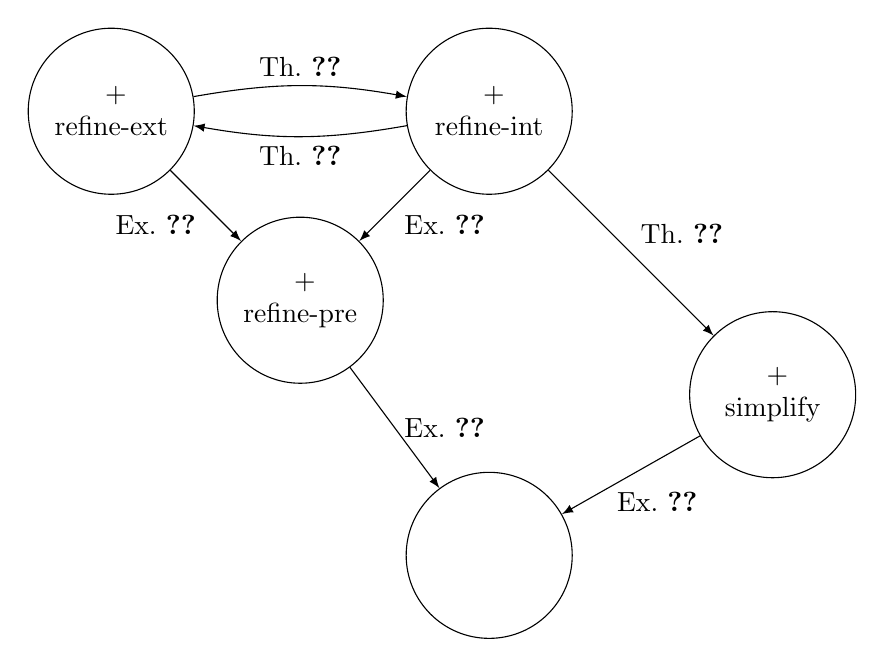
\begin{tikzpicture}[scale=1.2]
		\node[draw,circle,minimum size=6em] (LCL) at (0, -0.2) {$\LCLA$};
		\node[draw,circle,minimum size=6em,align=center] (RefPre) at (-2, 2.5) {$\LCLA$ + \\ \lclrule{refine\mbox{-}pre}};
		\node[draw,circle,minimum size=6em,align=center] (RefInt) at (0,4.5) {$\LCLA$ + \\ \lclrule{refine\mbox{-}int}};
		\node[draw,circle,minimum size=6em,align=center] (RefExt) at (-4,4.5) {$\LCLA$ + \\ \lclrule{refine\mbox{-}ext}};
		\node[draw,circle,minimum size=6em,align=center] (Simpl) at (3,1.5) {$\LCLA$ + \\ \lclrule{simplify}};

		\draw[-latex] (RefPre) edge [right] node {Ex.~\ref{ex:lcla:refine-pre-usefulness}} (LCL);
		\draw[-latex] (Simpl) edge [below right] node[shift={(-0.3,-0.1)}] {Ex.~\ref{ex:lcla:simplify-stronger}} (LCL);
		\draw[-latex] (RefExt) edge [below left] node {Ex.~\ref{ex:lcla:refine-pre-incomplete}} (RefPre);
		\draw[-latex] (RefExt) edge [bend left=10,above] node {Th.~\ref{th:lcla:refinement-rule-completeness}} (RefInt);
		\draw[-latex] (RefInt) edge [bend left=10,below] node {Th.~\ref{th:lcla:refine-int-completeness}} (RefExt);
		\draw[-latex] (RefInt) edge [below right] node {Ex.~\ref{ex:lcla:refine-pre-incomplete}} (RefPre);
		\draw[-latex] (RefInt) edge [above right] node {Th.~\ref{th:lcla:refine-int-completeness}} (Simpl);
	\end{tikzpicture}
	\caption{Relations between the new proof systems}\label{fig:lcla:rules-comparison-graph}
\end{figure}

We present a pictorial comparison among the expressiveness of the various proof systems in Figure~\ref{fig:lcla:rules-comparison-graph}. The bottom node of the diagram represents the original proof system $\LCLA$. Each other node represents the proof system extended with the single rule mentioned in the balloon. Each arrow corresponds to an expressivity result: all triples provable in the target system are also provable in the source system, which is thus more powerful. The labels reference the result that justifies the claim. For simplicity, we omit arrows obtained by transitivity. The two mutual arrows between the two topmost nodes indicate that the two proof systems are logically equivalent (i.e., they can prove the same triples).

%\begin{table}[t]
%	\caption{Comparison of the proof systems}
%	\label{tab:lcla:rules-comparison-table}
%	\centering
%	\renewcommand{\arraystretch}{1.5}
%	\setlength{\tabcolsep}{0.6em}
%	\begin{tabular}{c|c|c}
%		Proof system                          & Extensional & Logical completeness \\ \hline \hline
%		Plain $\LCLA$                         & \ding{55}   & \ding{55}            \\ \hline
%		$\LCLA$ + \lclrule{refine\mbox{-}ext} & \checkmark  & \checkmark           \\ \hline
%		$\LCLA$ + \lclrule{refine\mbox{-}int} & \checkmark  & \checkmark           \\ \hline
%		$\LCLA$ + \lclrule{refine\mbox{-}pre} & \checkmark  & \ding{55}            \\ \hline
%		$\LCLA$ + \lclrule{simplify}          & \ding{55}   & \ding{55}            \\
%	\end{tabular}
%\end{table}
%
%We also summarises the properties $\LCLA$ enjoys when extended with different rules in Table~\ref{tab:lcla:rules-comparison-table}.
%\lclrule{refine\mbox{-}ext} is the most general refinement rule, from which the other two \lclrule{refine\mbox{-}int} and \lclrule{refine\mbox{-}pre} are derived. The former turns out to be as strong as \lclrule{refine\mbox{-}ext}, since they are both logically complete, while the latter is simpler to use, although weaker.
%The only simplification rule \lclrule{simplify} is theoretically slightly stronger than plain $\LCLA$, given its intrinsic incompleteness, but it can prove triples which are not provable using \lclrule{refine\mbox{-}pre}, and it may be useful in practice.

%\subsection{Future works}
%While the new rules we introduced are relevant from both a theoretical and practical point of view, they do not define an algorithm because of their nondeterminism:
%% In principle, they may be applied to prove every triple moving to any refinement of the abstract domain, so
%we need techniques to determine \emph{when} a change of abstract domain is needed and \emph{how} to choose the most convenient new domain.
%We believe these two issues are actually related. For instance, if the analysis is unable to satisfy a local completeness proof obligation to apply \lclrule{transfer}, an heuristics may determine both what additional information is needed to make it true (i.e., how to refine the abstract domain) and where that additional information came from (i.e., when to refine). We briefly discussed in Section~\ref{sec:lcla:choose-refinement} some possibilities to perform this choice.
%Ideally, one would systematically select an off-the-shelf abstract domain best suited to deal with each code fragment and the heuristic would inspect the proof obligations, and exploit some sort of catalogue that can track suitable abstract domains that are locally complete for the code and input at hand or derive on-the-fly some convenient domain refinement as done, e.g., by partition refinement.
%To this aim, we intend to investigate a mutual exchange of ideas between CEGAR and our approach, and to integrate abstract interpretation repair into our framework.
